\documentclass{article}
\usepackage{amsmath}
\usepackage{amsfonts}
\usepackage{sectsty}
\usepackage{hyperref}
\usepackage{fancyhdr}
%TODO: FIX MARGINS
\usepackage[top=1in,bottom=1in,left=1in,right=1in]{geometry}
\usepackage{float}
\usepackage{graphicx}
\usepackage{tabularx}

\title{Lecture 2 - Discrete Systems}
\author{Matthew Farah, \href{mailto:farahm11@mcmaster.ca}{$\langle$farahm11@mcmaster.ca$\rangle$}, 400468251}
\date{\today}

\fancyhead{}
\fancyhead[L]{Matthew Farah, \href{mailto:farahm11@mcmaster.ca}{$\langle$farahm11@mcmaster.ca$\rangle$}, 400468251}
\fancyhead[R]{Lecture 2 - Discrete Systems}

\renewcommand{\thesubsection}{\thesection.\alph{subsection}}
\renewcommand{\thesubsubsection}{\thesection.\alph{subsection}.\Roman{subsubsection}}
\makeatletter

\newcolumntype{Y}{>{\centering\arraybackslash}X}
\renewcommand{\arraystretch}{1.8}

\sectionfont{\fontsize{12}{12}\bfseries}
\subsectionfont{\fontsize{10}{12}\normalfont}
\subsubsectionfont{\fontsize{10}{12}\normalfont}

\begin{document}
\maketitle

\begin{itemize}
	\item The \emph{steady state} of a system is the long term behaviour of a system's outputs.
\end{itemize}

\section[Example ~\thesection]{Compute the outputs to the Finite Impulse Response (FIR) system $y(n) = x(n) + x(n-2)$ for the following inputs:}

\subsection[~\thesubsection]{$x(n) = \cos(\frac{1}{2}{\pi}n)$}

\begin{tabularx}{\linewidth}{| c || Y Y Y Y Y Y |}
	\hline
	$n$ & 0 & 1 & 2 & 3 & 4 & 5 \\
	\hline
	$x(n)$ & 1 & 0 & -1 & 0 & 1 & 0 \\
	$y(n)$ & 1 & 0 & 0 & 0 & 0 & 0 \\
	\hline
\end{tabularx}

\vspace{.3cm}

Here, we can observe that the system's steady state is 0.

\subsection[~\thesubsection]{$x(n) = \cos({\pi}n)$}

\begin{tabularx}{\linewidth}{| c || Y Y Y Y Y Y |}
	\hline
	$n$ & 0 & 1 & 2 & 3 & 4 & 5 \\
	\hline
	$x(n)$ & 1 & -1 & 1 & -1 & 1 & -1 \\
	$y(n)$ & 1 & -1 & 2 & -2 & 2 & -2 \\
	\hline
\end{tabularx}

\vspace{.3cm}

Here we can observe that the system's steady state is $\pm2$.

Notice here that despite the difference equations being the same, $y(n)$'s steady state state differs depending on the frequency of the input cosine.

\vspace{.3cm}

\begin{itemize}
	\item Trying to evaluate what the steady-state behaviour of a system is by using the difference equation formula is largely fruitless.
	\begin{itemize}
		\item Expressing our input and output in terms of complex exponentials, is the key to understanding a system's steady state.
	\end{itemize}
	\item The complex exponential form for sine and cosine are given respectively as:
	\begin{align*}
		\sin({\omega}n) &= \frac{1}{2}(e^{i{\omega}n} + e^{-i{\omega}n}) \\
		\cos({\omega}n) &= \frac{1}{2i}(e^{i{\omega}n} - e^{-i{\omega}n})
	\end{align*}
\end{itemize}

\section[Example ~\thesection]{Compute the outputs to the system $y(n) = x(n) + x(n-2) \text{for the input} x(n) = e^{i{\omega}n}$}

\begin{align*}
	y(n) &= x(n) + x(n-2) \\
	&= e^{i{\omega}n} + e^{i{\omega}(n-2)} \\
	&= e^{i{\omega}n} + e^{i{\omega}n - 2i{\omega}} \\
	&= e^{i{\omega}n} + e^{i{\omega}n}e^{-2i{\omega}} \\
	&= (1 + e^{-2i{\omega}})e^{i{\omega}n}
\end{align*}

\vspace{.3cm}

\begin{itemize}
	\item From example 2, we can see that our output $y(n)$ is equal to our input $x(n) = e^{i{\omega}n}$ times some complex constant.
	\begin{itemize}
		\item This is generally true for all systems.
		\item This complex constant is called the system's \emph{frequency response}.
		\begin{itemize}
			\item Denoted $H(\omega)$
		\end{itemize}
	\end{itemize}
	\item In the same way that a system's impulse response, $h(n)$, describes a system's output when its input is the Kronecker-Delta function $x(n) = \delta(n)$, $H(\omega)$ describes a system's output when its input is a complex exponential $x(n) = e^{i{\omega}n}$.
		\item $H(\omega)$ describes how the system scales and phase-shifts complex exponential inputs.
\end{itemize}

\section[Example ~\thesection]{Evaluate the outputs to the system $y(n) = x(n) + x(n-2)$ for the following values of $\omega$:}

\subsection[~\thesubsection]{$\omega = \frac{1}{2}{\pi}$}

\begin{align*}
	y(n) &= (1 + e^{-2i{\omega}})e^{i{\omega}n} \\
	&= (1 + e^{-2i{(\frac{1}{2}\pi)}})e^{i{(\frac{1}{2}\pi)}n} \\
	&= (1 + e^{-{\pi}i})e^{\frac{1}{2}{\pi}in} \\
	&= (1 - 1)e^{\frac{1}{2}{\pi}in} \\
	&= 0
\end{align*}

\subsection[~\thesubsection]{$\omega = \pi$}

\begin{align*}
	y(n) &= (1 + e^{-2i{\omega}})e^{i{\omega}n} \\
	&= (1 + e^{-2i{(\pi)}})e^{i{(\pi)}n} \\
	&= (1 + e^{-2{\pi}i})e^{{\pi}in} \\
	&= (1 + 1)e^{{\pi}in} \\
	&= 2{(-1)}^n
\end{align*}

\vspace{.3cm}

Note that the outputs of these systems for complex exponentials whose frequencies corresspond to the angular frequencies of the cosines given in example 1 also correspond to their steady-state behaviour!

\newpage

\begin{center}
	\Large{\underline{Complex Numbers Recap}}
\end{center}

\begin{itemize}
	\item $i$ is defined to be $\sqrt{-1}$
	\begin{itemize}
		\item A complex number is any number $z$ which can be expressed as $z = a + bi$, where $a, b \in \mathbb{R}$.
		\begin{itemize}
			\item $\mathbb{R}$ denotes the set of all real numbers.
			\item $\mathbb{C}$ denotes the set of all complex numbers.
			\item $a$ is called the real component of $z$, $Re(z) = a$.
			\item $b$ is called the imaginary component of $z$, $Im(z) = b$.
			\item The complex conjugate of $z$ is defined as $a - bi$
			\begin{itemize}
				\item Denoted $\bar{z}$
			\end{itemize}
			\item the argument of $z$ is the angle formed between the vector pointing from the origin to z and the positive real axis in the complex plane.
			\begin{itemize}
				\item Denoted $arg(z)$
				\item For signals, the sign of $arg(z)$ is associated with being either forward or backwards in time.
			\end{itemize}
			\item The modulus of $z$ is the length of the vector pointing from the origin to $z$.
			\begin{itemize}
				\item Denoted $|z|$
				\item Given by $|z| = \sqrt{a^2 + b^2}$
			\end{itemize}
		\end{itemize}
	\end{itemize}
\end{itemize}

\begin{itemize}
	\item Some useful theorems:
	\begin{itemize}
		\item $Re(z) = \frac{1}{2}(z + \bar{z})$
		\item $Im(z) = \frac{1}{2}(z - \bar{z})$
	\end{itemize}
\end{itemize}

\begin{itemize}
	\item All exponential numbers, $z \in \mathbb{C}$ can be written in \emph{exponential form}.
	\begin{itemize}
		\item A complex number is in exponential form if it is some multiple of $e$ raised to some complex power.
		\item Given by $z = |z|e^{iarg(z)}$.
	\end{itemize}
\end{itemize}

\section{Express the following complex numbers in exponential form (with a negative argument)}

\subsection{$z = -i$}

\begin{figure}[H]
	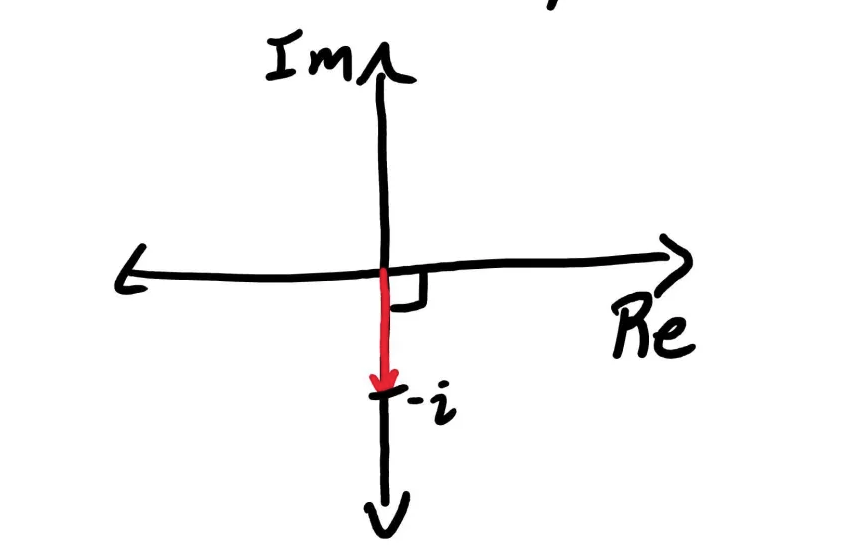
\includegraphics[width=\linewidth]{./imgs/Complex-Plane-1.png}
	\caption{$z$ in the complex plane}
\end{figure}

\begin{align*}
	|z| &= \sqrt{(a^2 + b^2)} \\
	&= \sqrt{(0^2 + (-1)^2)} \\
	&= \sqrt{1} \\
	&= 1 \\
	arg(z) &= \frac{-{\pi}}{2}
\end{align*}

Thus, $z = -i = e^{\frac{-{\pi}}{2}i}$

\subsection{$z = 1 + i$}

\begin{figure}[H]
	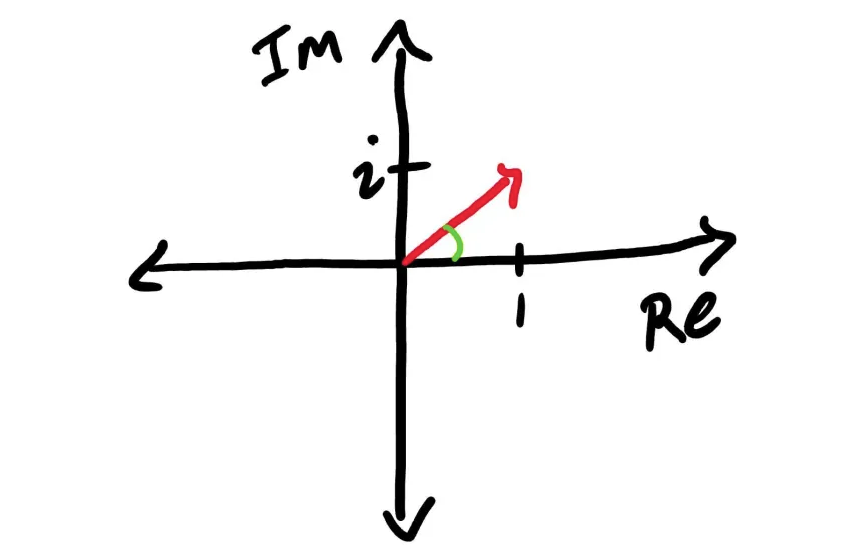
\includegraphics[width=\linewidth]{./imgs/Complex-Plane-2.png}
	\caption{$z$ in the complex plane}
\end{figure}

\begin{align*}
	|z| &= \sqrt{(a^2 + b^2)} \\
	&= \sqrt{(1^2 + 1^2)} \\
	&= \sqrt{2} \\
	arg(z) &= \frac{-7{\pi}}{4}
\end{align*}

Thus $z = 1 + i = \sqrt{2}e^{\frac{-7{\pi}}{4}i}$












































































































































\end{document}
